% Gemini theme
% https://github.com/anishathalye/gemini
%
% We try to keep this Overleaf template in sync with the canonical source on
% GitHub, but it's recommended that you obtain the template directly from
% GitHub to ensure that you are using the latest version.

\documentclass[final]{beamer}

% ====================
% Packages
% ====================


\newcommand{\off}{\operatorname{off}}
\newcommand{\on}{\operatorname{on}}
\newcommand{\gX}{\mathcal{X}}
\newcommand{\gA}{\mathcal{A}}
\newcommand{\gS}{\mathcal{S}}
\newcommand{\gF}{\mathcal{F}}
\newcommand{\gT}{\mathcal{T}}
\newcommand{\gL}{\mathcal{L}}
\newcommand{\Reg}{\text{Reg}}
\usepackage[T1]{fontenc}
\usepackage{boldline}
\usepackage{lmodern}
\usepackage[size=custom,width=36,height=24,scale=1]{beamerposter}
\usetheme{gemini}
\usecolortheme{gemini}
\usepackage{natbib}
\usepackage{graphicx}
\usepackage{booktabs}
\usepackage{tikz}
\usepackage{pgfplots}
\usepackage{verbatim}
%%%%% NEW MATH DEFINITIONS %%%%%
\usepackage{amsmath,bbm,bm}
\usepackage{amssymb}
\usepackage{amsfonts}
\usepackage{amsthm}
\usepackage{mathtools}

% commands
% global count (no section number)
\newtheorem{thm}{Theorem}%[section]
\newtheorem{lem}{Lemma}
\newtheorem{prop}{Proposition}
\newtheorem{cor}{Corollary}
\newtheorem{conj}{Conjecture}
\newtheorem{aspt}{Assumption}
\newtheorem{claim}{Claim}
\newtheorem{rmk}{Remark}
\newtheorem{commt}{Comment}
\newtheorem{defn}{Definition}

% algorithm
%\usepackage{algorithm, algorithmic}
%\usepackage{algorithm2e}
\usepackage{tabularx}
%\usepackage[table,xcdraw]{xcolor}

% Comments
% \usepackage{xcolor} % already loaded
\newcount\comments  % 0 suppresses notes to selves in text
\comments=1  % TODO: change to 0 for final version
\newcommand{\genComment}[2]{\ifnum\comments=1{\textcolor{#1}{\textsf{\footnotesize #2}}}\fi}
\newcommand{\ed}[1]{\genComment{red}{[EI:#1]}}
\newcommand{\giles}[1]{\genComment{green}{[GH:#1]}}
\newcommand{\kevin}[1]{\genComment{blue}{[KT:#1]}}


% Mark sections of captions for referring to divisions of figures
\newcommand{\figleft}{{\em (Left)}}
\newcommand{\figcenter}{{\em (Center)}}
\newcommand{\figright}{{\em (Right)}}
\newcommand{\figtop}{{\em (Top)}}
\newcommand{\figbottom}{{\em (Bottom)}}
\newcommand{\captiona}{{\em (a)}}
\newcommand{\captionb}{{\em (b)}}
\newcommand{\captionc}{{\em (c)}}
\newcommand{\captiond}{{\em (d)}}


\newcommand\seq[2]{{#1}\!:\!{#2}}
\newcommand\R{\mathbb{R}}
\newcommand\Var{\mathrm{Var}}
\newcommand\var{\Var}
\newcommand\Cov{\mathrm{Cov}}
\newcommand\cov{\Cov}
\newcommand\iid{\mathrm{iid}}
\newcommand\dist{d}
\newcommand\lik{\mathcal{L}}
\newcommand\prob{\mathbb{P}}
\newcommand\E{\mathbb{E}}
\newcommand\loglik{\ell}
\newcommand\process{\texttt{process}}
\newcommand\dimtheta{\mathrm{dim}_{\Theta}}
\newcommand\param{\,;}
\newcommand\giventh\param
\newcommand\given{{\,\vert\,}}
\newcommand\code[1]{\texttt{#1}}
\newcommand\ceil[1]{\lceil #1 \rceil}
\newcommand\floor[1]{\lfloor #1 \rfloor}
\newcommand\1{\bm{1}}


% Highlight a newly defined term
\newcommand{\newterm}[1]{{\bf #1}}


% Figure reference, lower-case.
\def\figref#1{figure~\ref{#1}}
% Figure reference, capital. For start of sentence
\def\Figref#1{Figure~\ref{#1}}
\def\twofigref#1#2{figures \ref{#1} and \ref{#2}}
\def\quadfigref#1#2#3#4{figures \ref{#1}, \ref{#2}, \ref{#3} and \ref{#4}}
% Section reference, lower-case.
\def\secref#1{section~\ref{#1}}
% Section reference, capital.
\def\Secref#1{Section~\ref{#1}}
% Reference to two sections.
\def\twosecrefs#1#2{sections \ref{#1} and \ref{#2}}
% Reference to three sections.
\def\secrefs#1#2#3{sections \ref{#1}, \ref{#2} and \ref{#3}}
% Reference to an equation, lower-case.
\def\eqref#1{equation~\ref{#1}}
% Reference to an equation, upper case
\def\Eqref#1{Equation~\ref{#1}}
% A raw reference to an equation---avoid using if possible
\def\plaineqref#1{\ref{#1}}
% Reference to a chapter, lower-case.
\def\chapref#1{chapter~\ref{#1}}
% Reference to an equation, upper case.
\def\Chapref#1{Chapter~\ref{#1}}
% Reference to a range of chapters
\def\rangechapref#1#2{chapters\ref{#1}--\ref{#2}}
% % Reference to an algorithm, lower-case.
% \def\algref#1{algorithm~\ref{#1}}
% % Reference to an algorithm, upper case.
% \def\Algref#1{Algorithm~\ref{#1}}
% \def\twoalgref#1#2{algorithms \ref{#1} and \ref{#2}}
% \def\Twoalgref#1#2{Algorithms \ref{#1} and \ref{#2}}
% Reference to a part, lower case
\def\partref#1{part~\ref{#1}}
% Reference to a part, upper case
\def\Partref#1{Part~\ref{#1}}
\def\twopartref#1#2{parts \ref{#1} and \ref{#2}}

\def\eps{{\epsilon}}

\def\gN{{\mathcal{N}}}
\def\gX{{\mathcal{X}}}
\def\gY{{\mathcal{Y}}}


\makeatletter
\newcommand*{\addFileDependency}[1]{% argument=file name and extension
\typeout{(#1)}% latexmk will find this if $recorder=0
% however, in that case, it will ignore #1 if it is a .aux or 
% .pdf file etc and it exists! If it doesn't exist, it will appear 
% in the list of dependents regardless)
%
% Write the following if you want it to appear in \listfiles 
% --- although not really necessary and latexmk doesn't use this
%
\@addtofilelist{#1}
%
% latexmk will find this message if #1 doesn't exist (yet)
\IfFileExists{#1}{}{\typeout{No file #1.}}
}\makeatother

\newcommand*{\myexternaldocument}[1]{%
\externaldocument{#1}%
\addFileDependency{#1.tex}%
\addFileDependency{#1.aux}%
}
%\usepackage{enumitem}

\usepackage[skins,theorems]{tcolorbox}
%\tcbset{colback=white}

\definecolor{ballblue}{rgb}{0.13, 0.67, 0.8}
\definecolor{darkred}{RGB}{139,0,0}

\tcbset{highlight math style={enhanced,colframe=red,colback=white}}

\usepackage{colortbl} % Add this package to use \cellcolor
\definecolor{lightgreen}{rgb}{0.9, 1, 0.9} % Light green color definition


\pgfplotsset{compat=1.14}

% ====================
% Lengths
% ====================

% If you have N columns, choose \sepwidth and \colwidth such that
% (N+1)*\sepwidth + N*\colwidth = \paperwidth

\setlength{\paperwidth}{36in}
\setlength{\paperheight}{24in}


\newlength{\sepwidth}
\newlength{\colwidth}
\setlength{\sepwidth}{0.025\paperwidth}
\setlength{\colwidth}{0.3\paperwidth}

\newcommand{\separatorcolumn}{\begin{column}{\sepwidth}\end{column}}

\newcommand{\cross}[1][1pt]{\ooalign{%
  \rule[1ex]{1ex}{#1}\cr% Horizontal bar
  \hss\rule{#1}{.7em}\hss\cr}}% Vertical bar

% ====================
% Title
% ====================

\title{Automatic differentiation accelerates inference
for partially-observed Markov processes}

\author{Kevin Tan \inst{*} \and Giles Hooker \inst{*} \and Edward L. Ionides \inst{\cross[.4pt]$\cdot$}}

\institute[shortinst]{\inst{*} Department of Statistics and Data Science, University of Pennsylvania \quad  \inst{\cross[.4pt]} Department of Statistics, University of Michigan}

% ====================
% Footer (optional)
% ====================

\footercontent{
  \hfill
   \hfill
  }
% (can be left out to remove footer)

% ====================
% Logo (optional)
% ====================

% use this to include logos on the left and/or right side of the header:
 %\logoright{\includegraphics[scale=0.24]{logo1.png}}
%\logoleft{\includegraphics[scale=2.5]{sci logo.png}}

% ====================
% Body
% ====================

\begin{document}

\begin{frame}[t]
\begin{columns}[t]
\separatorcolumn

\begin{column}{\colwidth}

  \begin{block}{Introduction}
  
\textbf{Inference for continuous-time, continuous-state hidden Markov models.}

\begin{tcolorbox}[enhanced,colback=white!100!white,colframe=red!100!red]
\textbf{\textcolor{red}{Partially-Observed Markov Process (POMP)}}: 
\begin{itemize}
    \item Unknown Markov process $\{X_t, t \geq t_0\}$, but we have observations $y_1^*,...,y_N^*$ at timesteps $t_1,..., t_N$.  
    \item Given measurements $y_n^*$, estimate both the latent state of the system $x_n$ at timesteps $t_0,...,t_N$ and system parameters $\theta \in \Theta$. 
\end{itemize}
\end{tcolorbox}
e.g. given monthly cholera case counts, estimate number of infected and recovered people in the population, and how transmissible the disease is. 

  \end{block}

  \vspace{-1ex}
  \begin{block}{Problem}
  \vspace{-1.6ex}
  \begin{tcolorbox}[enhanced,colback=white!100!white,colframe=red!100!red]
  \begin{center}
  Maximum likelihood with only a simulator, cannot evaluate $f_{X_n|X_{n-1};\theta}$. \textbf{Cannot use the EM algorithm!}
  \end{center}
\end{tcolorbox}

  \textbf{What to do now?} Particle filters provide a Monte Carlo approximation of the \textbf{filtering distribution} $f_{X_n|Y_{1:n};\theta}$ and the \textbf{log-likelihood} $\ell(\theta)$ increasingly accurate in the number of particles $J$. 
  
  \textbf{Gradient descent} using autodiff (AD) on the likelihood estimate? \textcolor{red}{But:}
  \begin{enumerate}
      \item Likelihood estimate not differentiable due to Monte Carlo resampling.
      \item Previous work \cite{corenflos21, naesseth18, scibior21} on this, but computationally expensive \cite{corenflos21}, has uncontrolled asymptotic bias \cite{naesseth18}, or has high variance \cite{poyiadjis11}. 
  \end{enumerate}
  \end{block}
  
  \begin{alertblock}{Solution: Off-Parameter Resampling}

    \textbf{Reconstruct likelihood} at $\theta$ by cumulatively reweighting particles resampled at a \textbf{baseline parameter} $\phi \in \Theta$. Take gradient at $\theta=\phi$.

    When treating the particles at $\phi$ as constants, you're now differentiating through (1) a differentiable simulator and (2) a series of measurement density ratios, so the resulting likelihood estimate is smooth!

    \textbf{Bias-variance tradeoff:} Discount cumulative reweighting by $\alpha \in [0,1]$.

  \end{alertblock}

  \vspace{-1ex}
    \begin{figure}
        \centering
        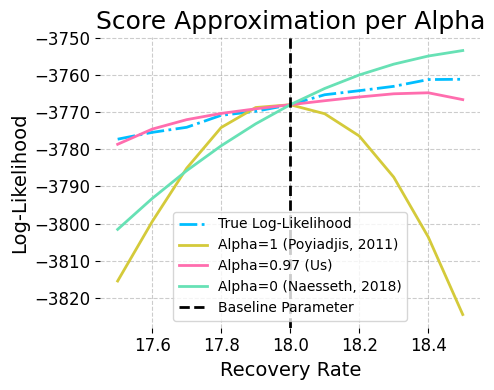
\includegraphics[width=0.45\linewidth]{imgs/095/mop.png}
        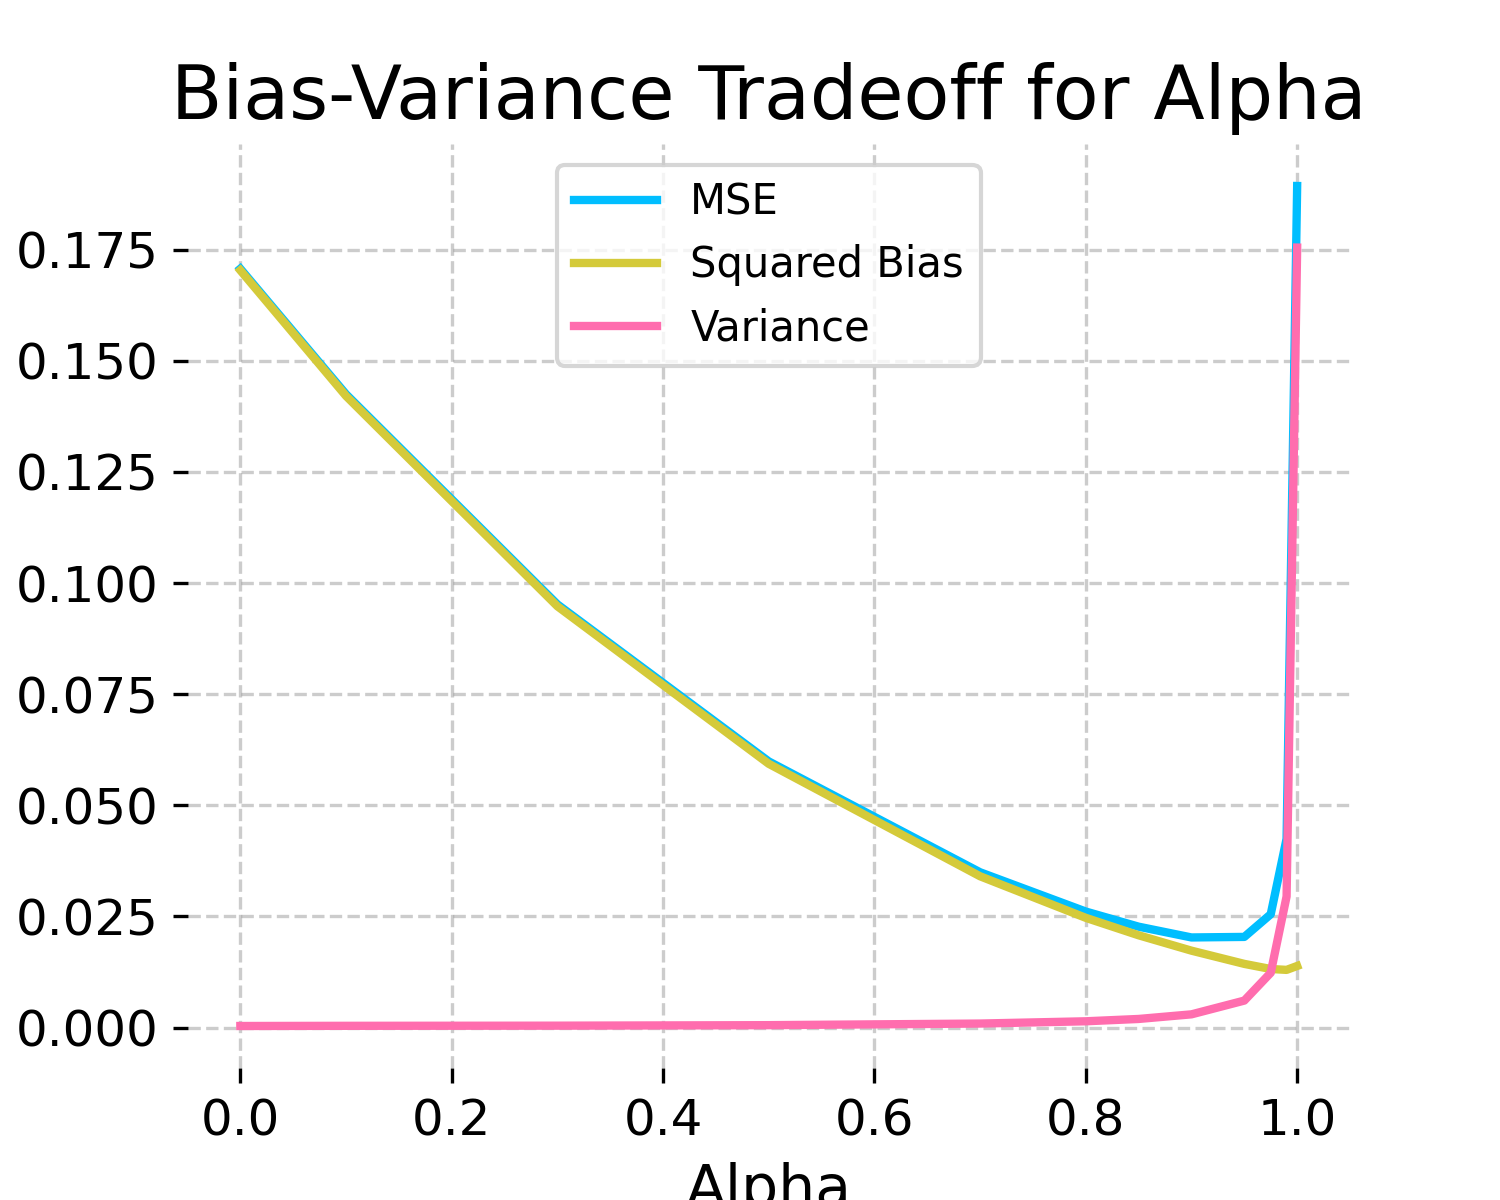
\includegraphics[width=0.405\linewidth]{imgs/095/biasvar.png}
        \caption{Dhaka cholera model of \cite{king08}. \textbf{Left:} Likelihood slice for the recovery rate parameter, and smooth off-parameter reconstructions for different $\alpha$. \textbf{Right:} Bias-variance tradeoff induced by $\alpha$ for estimation of the score for the trend parameter. }
        \label{fig:enter-label}
    \end{figure}
    
%Only simulation-based method for maximum likelihood available \cite{ionides15} gets close (\~40 nats) to the MLE quickly, but fails to find it ($\geq 7$ nats away). 

% \vspace{0.5em}
%  \begin{alertblock}{tl;dr}
    
%     \begin{itemize}
%         \item Modified an optimistic algorithm for general function approximation algorithm called GOLF \cite{jin2021bellmaneluder, xie2022policy}. 
%         \item Including the offline dataset in parameter estimation achieves provable improvements in regret over pure offline/online learning. 
%         \vspace{0.5ex}
%         \item How? Consider {\it arbitrary} (not necessarily disjoint) partitions of the state-action space $\gX_{\off} \cup \gX_{\on} = \gX$.
%         \begin{itemize}
%             \item Bound regret by the coverage of the behavior policy on $\gX_{\off}$  and a complexity measure for online learning on $\gX_{\on}$.
%             \item Overall regret is characterized by the regret bound on the best possible partition -- even if the algorithm is unaware of it. 
%         \end{itemize}
%         \item Not specific to DISC-GOLF! Yields a general recipe for initializing generic online RL algorithms with offline data without full coverage.
%     \end{itemize}

%   \end{alertblock}

\end{column}


\separatorcolumn

\begin{column}{\colwidth}

  \begin{alertblock}{Guarantees}

  \textbf{Correctness:} This procedure targets the filtering distribution, $\pi_n(\theta) = f_{X_n|Y_{1:n}}(x_n|y_{1:n}^*;\theta)$, and is strongly consistent for the likelihood under $\theta$. 
  We obtain a set of state estimates $(x_{n,j}^{F,\theta})_{j=1}^J$ and a likelihood estimate $\hat \lik_J(\theta)$ so for any $\alpha\in[0,1]$, for any measurable bounded functional $h$:
  $$\frac{\sum_{j=1}^J h\left(x_{n, j}^{F, \theta}\right) w_{n, j}^{F, \theta}}{\sum_{j=1}^J w_{n, j}^{F, \theta}} \stackrel{\text{a.s.}}{\to} E_{\pi_n(\theta)}\left[h\left(X_n\right)\right], \; \hat{\mathcal{L}}_J^\alpha(\theta) \stackrel{\text{a.s.}}{\to} \mathcal{L}(\theta) \text{ as } J \to \infty.$$

  \textbf{Consistent score estimates:} When $\alpha=1$, $\nabla_\theta \hat\ell_J^1(\theta) \stackrel{\text{a.s.}}{\to} \ell(\theta)$ as $J \to \infty$. Else, increasing asymptotic bias as $\alpha \to 0$ in return for lower variance.

  \textbf{Encompasses other estimators:} When $\alpha=0$, $\nabla_\theta \hat\ell_J^0(\theta)$ is equivalent to the low-variance but asymptotically biased estimate of \cite{naesseth18}. When $\alpha=1$, $\nabla_\theta \hat\ell_J^1(\theta)$ is equivalent to the high-variance but consistent estimate of \cite{poyiadjis11}.

  \end{alertblock}

  \vspace{-2ex}
  \begin{block}{Rates}
  \vspace{-6.5mm}
      \begin{table}[t]
\centering
\scalebox{0.85}{
\begin{tabular}{c  c}
\toprule & MSE 
\tabularnewline
\toprule 
\vspace{0.2ex}
$\alpha \in (0,1)$ & $\tcbhighmath[colframe=ballblue]{\min_{k \leq N} N p G^{\prime}(\theta)^2(k^2/J+(1-\epsilon)^{\lfloor k /(c \log (J))\rfloor}+k+\psi_k(\alpha))}$
\vspace{0.2ex}
\tabularnewline \hline
\vspace{0.2ex}
$\alpha=0$, equivalent to \cite{naesseth18} & $N p G'(\theta)^2(J^{-1} + (1-\epsilon)^{\lfloor 1 /(c \log (J))\rfloor})$
\vspace{0.2ex}
\tabularnewline
\hline
\vspace{0.2ex}
$\alpha=1$, equivalent to \cite{poyiadjis11} & $N^4pG'(\theta)^2/J$
\vspace{0.2ex}
\tabularnewline
\toprule
&  Variance
\tabularnewline
\toprule\vspace{0.2ex}
$\alpha \in (0,1)$ & $\tcbhighmath[colframe=ballblue]{\min _{k \leq N}\left(\frac{k^2 p G^{\prime}(\theta)^2 N p}{(1-\alpha)^2 J}+\frac{\alpha^k}{1-\alpha} N p G^{\prime}(\theta)^2\right)}$
\vspace{0.2ex}
\tabularnewline \hline
\vspace{0.2ex}
$\alpha=0$, equivalent to \cite{naesseth18} & $N p G'(\theta)^2/J$
\vspace{0.2ex}
\tabularnewline
\hline
\vspace{0.2ex}
$\alpha=1$, equivalent to \cite{poyiadjis11} & $N^4pG'(\theta)^2/J$
\vspace{0.2ex}
\tabularnewline
\toprule 
\end{tabular}}
\medskip
\caption{Rates given the number of particles $J$, trajectory length $N$, dimension of parameter space $p$, bound on gradient norm $G'(\theta)$, and model-specific constant $\epsilon>0$. We define $\psi_k(\alpha)=\left(\alpha^k+\alpha^{k+1}-\alpha\right) /(1-\alpha)$. Our novel contribution of $\alpha \in (0,1)$ has a lower MSE than, and interpolates between the variances of, $\alpha=0$ \cite{naesseth18} and $\alpha=1$ \cite{poyiadjis11}.}
\label{tab:bounds}
\vspace{-5mm}
\end{table}
  \end{block}

\begin{block}{Practical Maximum Likelihood Estimation}
    \textbf{Problem:} Difficult, noisy, and nonconvex problem. Gradient descent/L-BFGS/Newton struggles with saddle points, local minima, and ridges.
    
    \textbf{Solution:} Warm-start gradient descent with IF2 algorithm of \cite{ionides15}. IF2 gets to a neighborhood of the MLE quickly, but fails to find it. Gradient descent does well in that neighborhood, warm-start achieves best of both worlds. 

    \textbf{Theoretical guarantee:} 

\end{block}


\end{column}

\separatorcolumn

\begin{column}{\colwidth}


  \begin{exampleblock}{Simulations: Hybrid RL Encourages Exploration}

  \textbf{Does appending the offline dataset to the experience replay buffer encourage sufficient exploration for the portion of the state-action space that does not have good coverage?}

  \textbf{Tabular:} Initialized UCBVI \cite{azar2017minimax} with an offline dataset of $100$ trajectories of length $20$ on a forest management simulator. 
  %Online partition is the state-action pairs with occupancy below $1/SA$.

\begin{figure}[H]
    \centering
    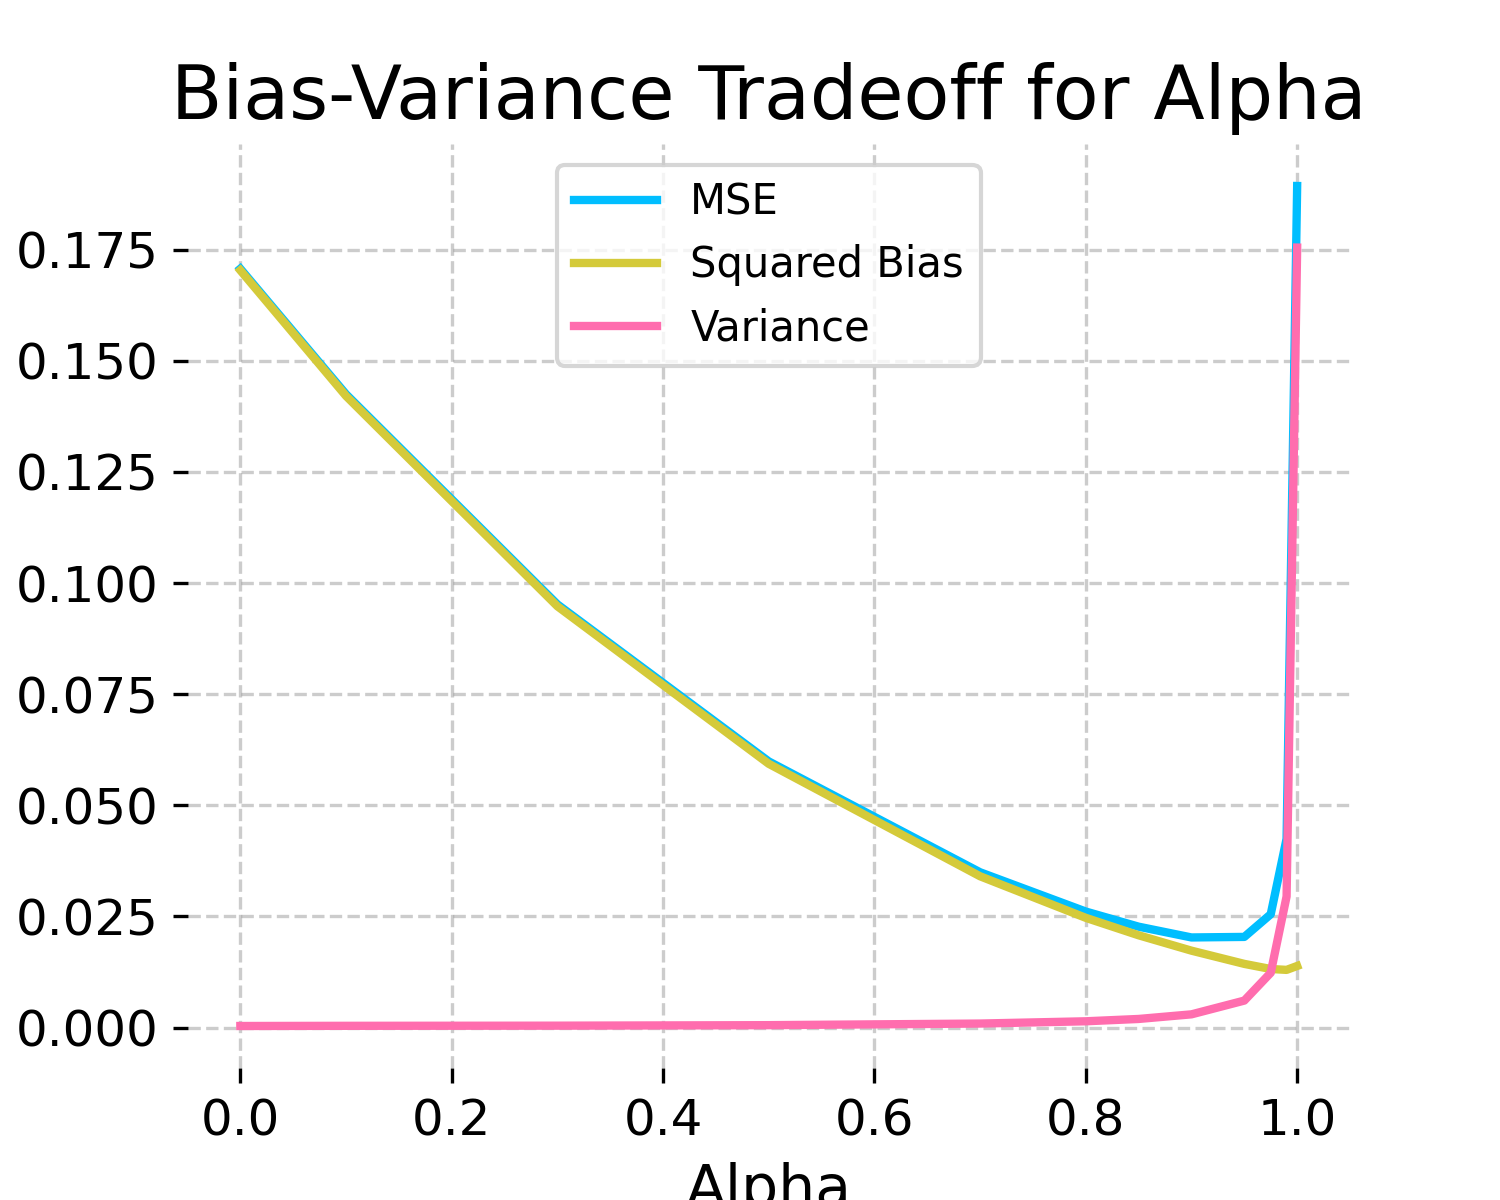
\includegraphics[scale=1]{imgs/095/biasvar.png}
    \caption{Hybrid RL explores more of the online partition (poorly covered $s,a$) to fill in the gaps in the offline dataset than online RL does, unless the behavior policy is optimal.
    }
\end{figure}

    \textbf{Linear:} Initialized LSVI-UCB \cite{jin2020provably} with $200$ trajectories of length $40$ on a scaled-down version of Tetris.

    \begin{figure}[H]
    \centering
    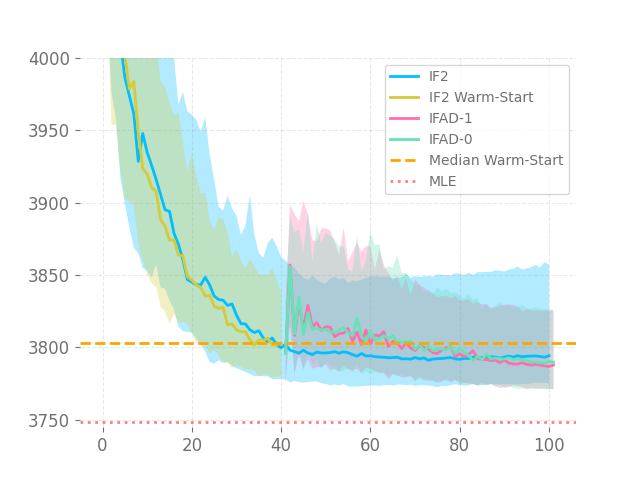
\includegraphics[scale=1]{imgs/095/optim.png}
    \caption{Hybrid RL takes fewer online episodes than online-only RL to achieve a lower concentrability coefficient.}
    \label{fig:linear-coverage}
\end{figure}


    
  \end{exampleblock}


\vspace{-2ex}
  
%\vskip-1ex
\begin{block}{}
  \vspace{-0.2em}
    \tiny{\bibliographystyle{plain}
    \bibliography{paper/bib-ifad}}
\end{block}



  %\vskip-1ex
  \vspace{0.2em}

  
  % \begin{block}{Contact Information}
  % \vskip-0ex
  %   %\nocite{*}
  %   \small{{Email Address}: kevtan@wharton.upenn.edu}
  % \end{block}

\end{column}

\separatorcolumn
\end{columns}
\end{frame}

\end{document}
